%\documentclass[tikz, border=5pt]{standalone}
\begin{document}
	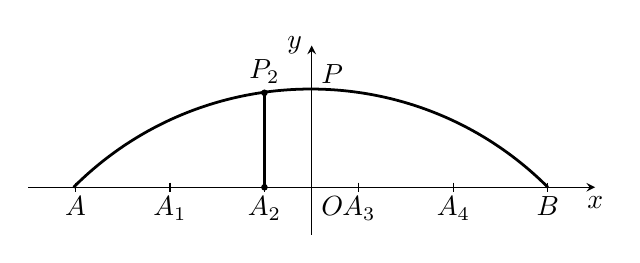
\begin{tikzpicture}[>=stealth, scale=0.6] % 箭头样式为stealth,
		
		% 绘制坐标轴
		\draw[->] (-6,0) -- (6,0) node[below] {$x$}; % x轴(带箭头和标签)
		\draw[->] (0,-1) -- (0,3) node[ left] {$y$}; % y轴(带箭头和标签)
		\node at (0,0) [below right] {$O$};           % 原点O的标签
		
		% 绘制所有小刻度线(从 -1 到 2,每隔 1 单位画竖线)
		\foreach \x in {-5,-3,...,5} {
			\draw (\x, 0.1) -- (\x, -0.1) ;  % 小竖线(长 0.2 单位)
		}
		
		% 绘制拱形
		\draw[line width=1pt] (5, 0) arc (45:135:7.1) ; 
		
		% 定义各关键点坐标
		\coordinate (A_2) at (-1,0);  % 点A₂
		\coordinate (P_2) at (-1,2); % 点P₂
		
		\draw[thick] (A_2) -- (P_2) ;
		
		% 标记各点的标签
		\fill (A_2) circle (2pt) node [below] {$A_2$};  % 带标签的实心点
		\fill (P_2) circle (2pt) node [above] {$P_2$};  % 带标签的实心点
		\node[below] at (-5,0) {$A$};
		\node[below] at (-3,0) {$A_1$};
		\node[below] at (1,0) {$A_3$};
		\node[below] at (3,0) {$A_4$};
		\node[below] at (5,0) {$B$};
		\node[above right] at (0,2) {$P$};
		
	\end{tikzpicture}
\end{document}
